
Note that in case of any changes in the SIZE file, a recompilation is necessary.\\
\subsection{Uniformly Distributed Mesh}

Suppose you wish to simulate flow through an axisymmetric pipe,
of radius \(R=0.5\) and length \(L=4\).  You estimate that you will
need 3 elements in radial (\(y\)) direction, and 5 in the \(x\) direction,
as depicted in Fig. \ref{fig:mesh_axi1}.
This would be specified by the following input file (called {\em pipe.box})
to genbox:

\begin{verbatim}
axisymmetric.rea
2                      spatial dimension
1                      number of fields
#
#    comments:   This is the box immediately behind the 
#                refined cylinder in Ugo's cyl+b.l. run.
#
#
#========================================================
#
Box 1                         Pipe
-5 -3                         Nelx  Nely
0.0   4.0   1.0               x0  x1   ratio
0.0   0.5   1.0               y0  y1   ratio
v  ,O  ,A  ,W  ,   ,          BC's:  (cbx0, cbx1, cby0, cby1, cbz0, cbz1)
\end{verbatim}
\begin{figure}
\centering
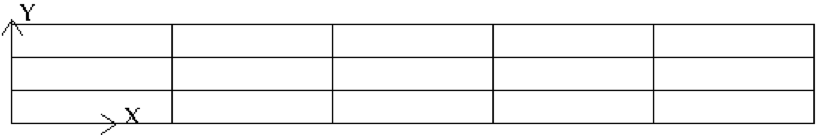
\includegraphics[width=0.8\textwidth]{mesh_axi1}
\caption{Axisymmteric pipe mesh}
\label{fig:mesh_axi1}
\end{figure}
\noindent
\begin{itemize}
\item
The first line of this file supplies the name of an existing 2D .rea file
that has the appropriate run parameters (viscosity, timestep size, etc.).
These parameters can be modified later, but it is important that 
axisymmetric.rea be a 2D file, and not a 3D file.
\item
The second line indicates the number of fields for this simulation, in
this case, just 1, corresponding to the velocity field (i.e., no heat 
transfer).
\item
The next set of lines just shows how one can place comments into a genbox
input file.
\item
The line that starts with ``Box'' indicates that a new box is starting,
and that the following lines describe a typical box input.  Other possible
key characters (the first character of Box, ``B'') are ``C'' and ``M'',
more on those later.
\item
The first line after ``Box'' specifies the number of elements in the
\(x\) and \(y\) directions.   The fact that these values are negative indicates
that you want genbox to automatically generate the element distribution 
along each axis, rather than providing it by hand.  (More on this below.)
\item
The next line specifies the distribution of the 5 elements in the \(x\) direction.
The mesh starts at \(x=0\) and ends at \(x=4.0\).  The {\em ratio} indicates the
relative size of each element, progressing from left to right.  Here, 
\item
The next line specifies the distribution of the 3 elements in the \(y\) direction,
starting at \(y=0\) and going to \(y=0.5\).  Again, 
{\em ratio}=1.0 indicates that the elements will be of uniform height.
\item
The last line specifies boundary conditions on each of the 4 sides of the
box:  
\begin{itemize}
\item
Lower-case {\em v} indicates that the left (\(x\)) boundary is to be a velocity
boundary condition, with a user-specified distribution determined by 
routine {\em userbc} in the .usr file.  (Upper-case \(V\) would indicate that
the velocity is constant, with values specified in the .rea file.)
\item
{\em O} indicates that the right (\(x\)) boundary is an outflow boundary -- the
flow leaves the domain at the left and the default exit pressure is \(p=0\).
\item
{\em A} indicates that the lower (\(y\)) boundary is the axis---this condition
is mandatory for the axisymmetric case, given the fact that the lower domain
boundary is at \(y=0\), which corresponds to \(r=0\).
\item
{\em W} indicates that the upper (\(y\)) boundary is a wall.  This would be
equivalent to a {\em v} or {\em V} boundary condition, with \(\bu=0\).
\end{itemize}
\end{itemize}


\subsection{Graded Mesh}
\begin{figure}
\centering
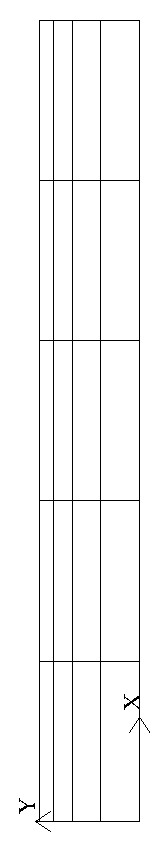
\includegraphics[width=0.8\textwidth]{mesh_axi2}
\caption{Axisymmteric pipe mesh, graded}
\label{fig:mesh_axi2}
\end{figure}

Suppose you wish to have the mesh be graded,
that you have increased resolution near the wall.
In this case you change {\em ratio} in the \(y\)-specification
of the element distribution.  For example, changing the 3 lines
in the above genbox input file from

\begin{verbatim}
-5 -3                         Nelx  Nely
0.0   4.0   1.0               x0  x1   ratio
0.0   0.5   1.0               y0  y1   ratio
\end{verbatim}

\noindent
to

\begin{verbatim}
-5 -4                         Nelx  Nely
0.0   4.0   1.0               x0  x1   ratio
0.0   0.5   0.7               y0  y1   ratio
\end{verbatim}

\noindent
yields the mesh shown in Fig. \ref{fig:mesh_axi2}.


\subsection{User-Specified Distribution}
\begin{figure}
\centering
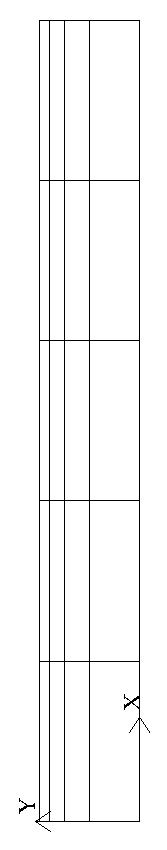
\includegraphics[width=0.6\textwidth]{mesh_axi3}
\caption{Axisymmteric pipe mesh, user specified}
\label{fig:mesh_axi3}
\end{figure}

You can also specify your own, precise, distribution of element
locations.   For example, another graded mesh similar to the
one of the preceding example could be built by changing the
genbox input file to contain:


\begin{verbatim}
-5  4                                               Nelx  Nely
0.0   4.0   1.0                                     x0  x1   ratio
0.000    0.250    0.375    0.450    0.500           y0  y1 ... y4
\end{verbatim}

\noindent
Here, the positive number of elements for the \(y\) direction indicates
that genbox is expecting {\tt Nely+1} values of \(y\) positions on the
\(y\)-element distribution line.   This is the genbox default, which
explains why it corresponds to {\tt Nely} \(>\) 0.  The corresponding mesh
is shown in Fig. \ref{fig:mesh_axi3}.


\subsection{Mesh Modification in Nek5000}

For complex shapes, it is often convenient to modify the mesh
direction in the simulation code, Nek5000.  This can be done
through the usrdat2 routine provided in the .usr file.
The routine usrdat2 is called by nek5000 immediately after
the geometry, as specified by the .rea file, is established.
Thus, one can use the existing geometry to map to a new geometry
of interest.

For example, suppose you want the above pipe geometry to have
a sinusoidal wall.  Let \(\bx := (x,y)\) denote the old geometry,
and \(\bx' := (x',y')\) denote the new geometry.  For a domain
with \(y\in [0,0.5]\), the following function will map the straight
pipe geometry to a wavy wall with amplitude \(A\), wavelength \(\lambda\):
\begin{eqnarray*}
y'(x,y) = y  + y A \sin( 2 \pi x / \lambda ).
\end{eqnarray*}
Note that, as \(y \longrightarrow 0\), the perturbation, 
\(yA \sin( 2 \pi x / \lambda )\), goes to zero.  So, near the axis,
the mesh recovers its original form.

In nek5000, you would specify this through usrdat2 as follows


\begin{verbatim}
      subroutine usrdat2
      include 'SIZE'
      include 'TOTAL'

      real lambda

      ntot = nx1*ny1*nz1*nelt

      lambda = 3.
      A      = 0.1

      do i=1,ntot
         argx         = 2*pi*xm1(i,1,1,1)/lambda
         ym1(i,1,1,1) = ym1(i,1,1,1) + ym1(i,1,1,1)*A*sin(argx)
      enddo

      param(59) = 1.  ! Force nek5 to recognize element deformation.

      return
      end
\end{verbatim}
\noindent
Note that, since nek5000 is modifying the mesh, postx will not
recognize the current mesh unless you tell it to, because postx
looks to the .rea file for the mesh geometry.  The only way for
nek5000 to communicate the new mesh to postx is via the .fld
file, so you must request that the geometry be dumped to the
.fld file.   This is done by modifying the OUTPUT SPECIFICATIONS,
which are found near the bottom of the .rea file.  Specifically,
change

\begin{verbatim}
  ***** OUTPUT FIELD SPECIFICATION *****
   6 SPECIFICATIONS FOLLOW
   F      COORDINATES
   T      VELOCITY
   T      PRESSURE
   T      TEMPERATURE
   F      TEMPERATURE GRADIENT
   0      PASSIVE SCALARS
\end{verbatim} 

\noindent
to

\begin{verbatim}
  ***** OUTPUT FIELD SPECIFICATION *****
   6 SPECIFICATIONS FOLLOW
   T      COORDINATES                       <------  CHANGE HERE
   T      VELOCITY
   T      PRESSURE
   T      TEMPERATURE
   F      TEMPERATURE GRADIENT
   0      PASSIVE SCALARS
\end{verbatim} 

\noindent
The result of above changes is shown in Fig. \ref{fig:wavypipe}.
\begin{figure}
\centering
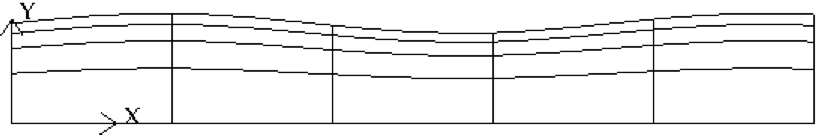
\includegraphics[width=0.8\textwidth]{wavypipe}
\caption{Axisymmteric pipe mesh}
\label{fig:wavypipe}
\end{figure}

\subsection{Cylindrical/Cartesian-transition Annuli}
\begin{figure}
\centering
\subfloat[Annuli mesh]{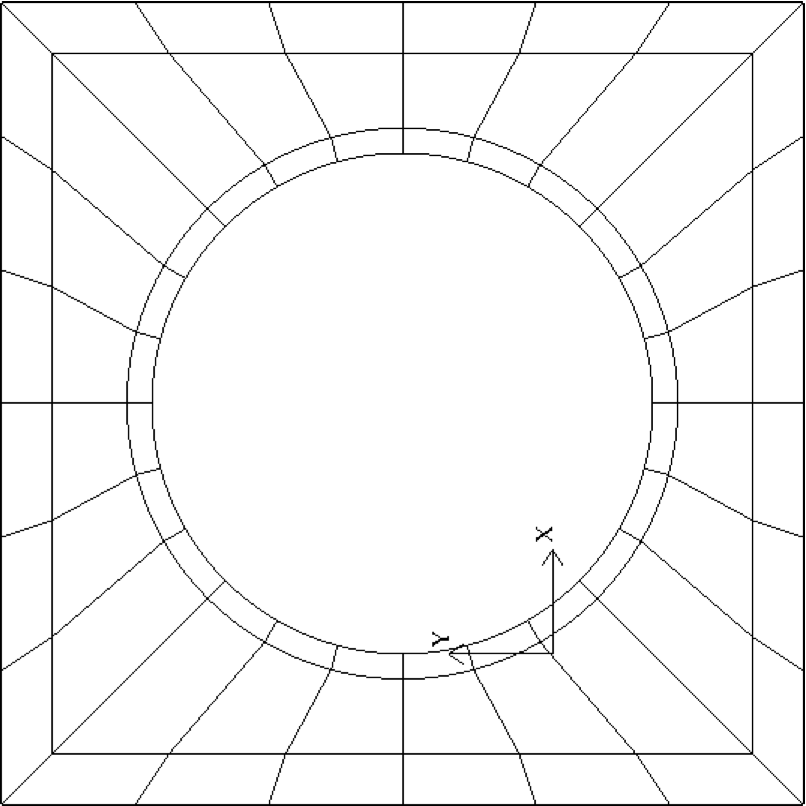
\includegraphics[width=0.3\textwidth]{cylbox_2d}\label{fig:cylbox_2d}}
\quad\quad\quad
\subfloat[Annuli mesh] {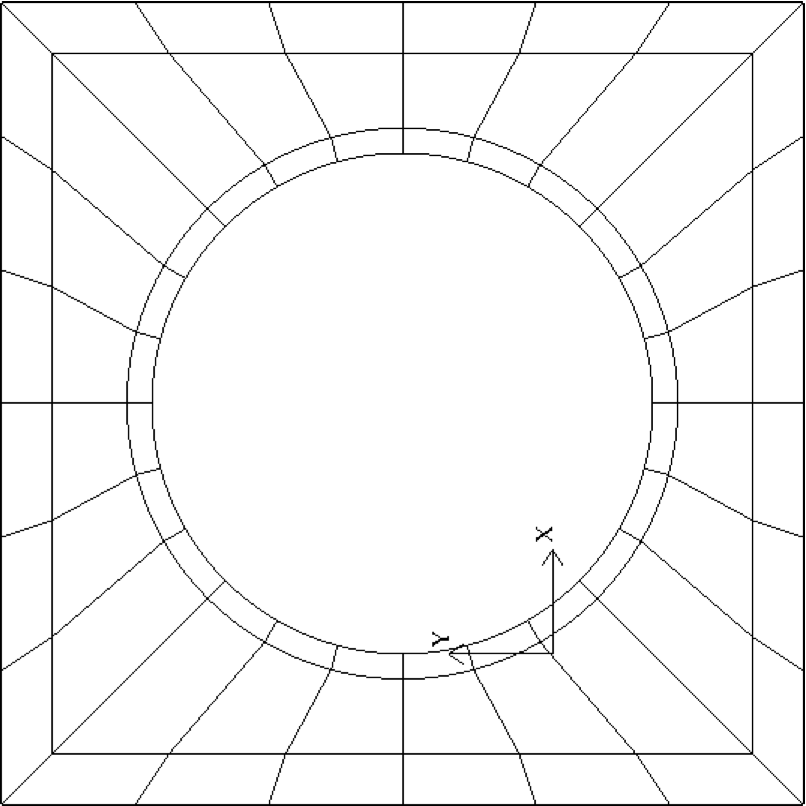
\includegraphics[width=0.3\textwidth]{cylbox_2d}\label{fig:cylbox_2da}} 
\caption{Cylinder mesh}
\end{figure}


An updated version of genb6, known as genb7, is currently under development
and designed to simply/automate the construction of cylindrical annuli, 
including {\em basic} transition-to-Cartesian elements.   More sophisticated
transition treatments may be generated using the GLOBAL REFINE options in
prenek or through an upgrade of genb7, as demand warrants.
Example 2D and 3D input files are provided in the nek5000/doc files
{\em box7.2d} and {\em box7.3d}.
Figure \ref{fig:cylbox_2d} shows a 2D example generated using 
the {\em box7.2d} input file, which reads:
\begin{verbatim}
x2d.rea
2                      spatial dimension
1                      number of fields
#
#    comments
#
#
#========================================================
#
Y                   cYlinder
3 -24 1             nelr,nel_theta,nelz
.5 .3               x0,y0 - center of cylinder
ccbb                descriptors: c-cyl, o-oct, b-box (1 character + space)
.5 .55 .7 .8        r0 r1 ... r_nelr
0  1  1             theta0/2pi theta1/2pi  ratio 
v  ,W  ,E  ,E  ,    bc's (3 characters + comma)
\end{verbatim}

\noindent
An example of a mesh is shown in Fig. \ref{fig:cylbox_2d}.   The mesh has been quad-refined
once with oct-refine option of prenek. The 3D counterpart to this 
mesh could joined to a hemisphere/Cartesian transition built with
the spherical mesh option in prenek. 
